\documentclass[10pt,openright,twoside,french]{book}

\input philippe2013
\input philippe2013_cours
\input philippe2013_sections
\input philippe2013_chapitre
\renewcommand\PartProgramme{Info. chiffrée}
\renewcommand\MaCouleur{Melon!150}

\pieddepage{}{%
\begin{tikzpicture}[scale=0.65]
\shadedraw [top color=white, bottom color=\MaCouleur, draw=\MaCouleur]
[l-system={Sierpinski triangle, step=1pt, angle=60, axiom=F, order=6.5}]
lindenmayer system -- cycle;
\draw (30:0.65cm) node {\bfseries\textcolor{black}{\thepage}};
\end{tikzpicture}%
}{}

\setcounter{chapter}{4}

\begin{document}
\chapter{Proportions}\label{ch_proportion}

\section{Vocabulaire}

\begin{Defi}
    \begin{enumerate}
        \item Une \ipt{population} $E$ est un ensemble d'éléments appelés les \ipt{individus} de cette population. Le nombre d'individus est appelé l'\ipt{effectif} de $E$, on le notera $n_E$.
        \item Une \ipt{sous-population} $A$ de $E$ est une population dont tous les individus sont aussi des individus de $E$.
    \end{enumerate}
\end{Defi}

\begin{Exemple}
    Tous les livres d'une bibliothèque constituent une population $B$. Les romans sont une sous-population de $B$.
\end{Exemple}

\begin{Defi}
    La \ipt{proportion} (ou \ipt{fréquence}) d'une sous-population $A$ dans une population $E$ est le nombre $p_A$ tel que :
    \[p_A = \frac{n_A}{n_E}.\]
    La population $E$ est la \iptb{population de référence}\index{population!de référence}.\par
    $p_A$ est aussi la proportion des individus de $A$ parmi les individus de $E$.
\end{Defi}

\begin{Rmq}
    Puisque $0 \leq n_A \leq n_E$, alors la proportion $p_A$ est toujours comprise entre $0$ et $1$.
\end{Rmq}

\begin{Exemple}
    Parmi les $\np{24000}$ votants d'une ville, $\np{18000}$ personnes ont voté pour Paul au second tour d'une élection.\par
    La population $E$ est composé des votants donc $n_E = \np{24000}$.\par
    La sous-population $A$ est composé des personnes ayant voté pour Paul donc $n_A = \np{18000}$.\par
    La proportion des voix obtenues par Paul est donc : \[p_A = \frac{n_A}{n_E} = \frac{\np{18000}}{\np{24000}} = \frac{18}{24} = \frac{3}{4} = 0,75 = 75\%.\]
\end{Exemple}

\section{Intersection et réunion de sous-populations}

Soient $A$ et $B$ deux sous-populations d'une même population $E$.

\begin{Defi}
    L'\ipt{intersection} de $A$ et $B$, notée $A \cap B$, est l'ensemble des individus de $E$ qui appartiennent à $A$ \textbf{et} à $B$.
\end{Defi}

\begin{center}
    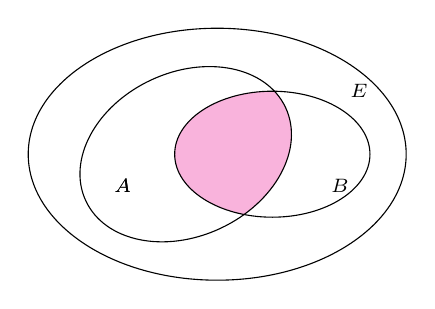
\begin{tikzpicture}[scale=0.4]
        \def\E{(1,0) ellipse (6 and 4); \draw (5.5,2) node {\scriptsize $E$};}
        \def\A{(0,0) ellipse (3.5 and 2.6); \draw (-2,-1) node {\scriptsize $A$};}
        \def\B{(2.75,0) ellipse (3.1 and 2); \draw (4.9,-1) node {\scriptsize $B$};}
        \begin{scope}
            \clip[rotate=25] \A;
            \fill[color=magenta!30] \B;
        \end{scope}
        \draw \E;
        \draw[rotate=25] \A;
        \draw \B;
    \end{tikzpicture}
\end{center}

\begin{Defi}
    La \ipt{réunion} de $A$ et $B$, notée $A \cup B$, est l'ensemble des individus de $E$ qui appartiennent à $A$ \textbf{ou} à $B$ de façon non exclusive.
\end{Defi}

\begin{center}
    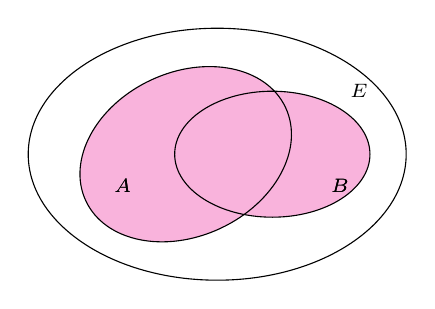
\begin{tikzpicture}[scale=0.4]
        \def\E{(1,0) ellipse (6 and 4); \draw (5.5,2) node {\scriptsize $E$};}
        \def\A{(0,0) ellipse (3.5 and 2.6); \draw (-2,-1) node {\scriptsize $A$};}
        \def\B{(2.75,0) ellipse (3.1 and 2); \draw (4.9,-1) node {\scriptsize $B$};}
        \fill[color=magenta!30,rotate=25] \A;
        \fill[color=magenta!30] \B;
        \draw \E;
        \draw[rotate=25] \A;
        \draw \B;
    \end{tikzpicture}
\end{center}

\begin{Exemple}
    On interroge $\np{1000}$ personnes qui constituent la population $E$.\par
    On note $A$ la sous population de $E$ des personnes qui possèdent un ordinateur et on note $B$ la sous-population de $E$ qui possède une télévision.\par
    Le tableau ci-dessous indique tous les résultats du sondage :\medskip
    
    \begin{center}
    \renewcommand\arraystretch{1.5}
        \begin{tabular}{|l|c|c|c|}
            \cline{2-4}
                \multicolumn{1}{c|}{} & Ont un ordinateur & N'ont pas d'ordinateur & Total \\
            \hline
                Ont une télévision & $345$ & $385$ & $730$ \\
            \hline
                N'ont pas de télévision & $75$ & $195$ & $270$ \\
            \hline
                Total & $420$ & $580$ & $\np{1000}$ \\
            \hline
        \end{tabular}
    \end{center}
    On a donc :
    \[n_E = \np{1000} \qq n_A = 420 \qq n_B = 730.\]
    $A \cap B$ représente ceux qui ont un ordinateur et un téléviseur donc : $n_{A\cap B} = 345$.\par
    $A \cup B$ représente ceux qui ont un ordinateur ou un téléviseur. On retire donc ceux qui n'ont ni ordinateur, ni téléviseur. Donc : $n_{A \cup B} = \np{1000} - 195 = 805$.
\end{Exemple}

\begin{Prop}
    $A$ et $B$ sont deux sous-populations d'une population $E$.\par
    Les proportions $p_A$, $p_B$, $p_{A \cap B}$ et $p{A \cup B}$ sont reliées par la relation suivantes :
    \[p_A + p_B = p_{A\cup B} + p_{A\cap B}.\]
\end{Prop}

\section{Inclusion}

\begin{Defi}
    On considère une population $E$ et une sous-population $A$ de $E$. Puisque tous les éléments de $A$ sont des éléments de $E$, on dit que $A$ est \iptb{inclus}\index{inclusion} dans $E$ et on note $A \subset E$.
\end{Defi}

\begin{center}
Ici, tous les éléments de $A$ sont dans $E$ donc $A \subset E$.\par En revanche, certains éléments de $B$ ne sont pas dans $E$ donc $B \not\subset E$.\medskip

    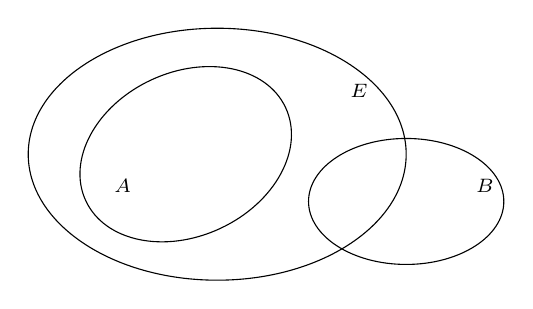
\begin{tikzpicture}[scale=0.4]
        \def\E{(1,0) ellipse (6 and 4); \draw (5.5,2) node {\scriptsize $E$};}
        \def\A{(0,0) ellipse (3.5 and 2.6); \draw (-2,-1) node {\scriptsize $A$};}
        \def\B{(7,-1.5) ellipse (3.1 and 2); \draw (9.5,-1) node {\scriptsize $B$};}
        \draw \E;
        \draw[rotate=25] \A;
        \draw \B;
    \end{tikzpicture}
\end{center}

\begin{Prop}
    Soit $E$ une population. On note $A$ une sous-population de $E$ et $B$ une sous-population de $A$.\medskip
    
\begin{center}
    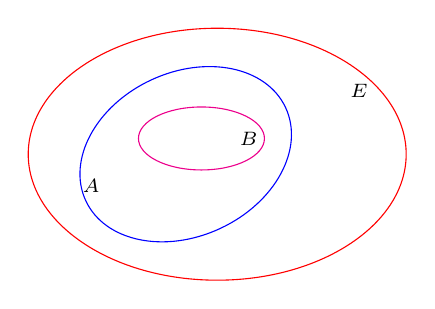
\begin{tikzpicture}[scale=0.4]
        \def\E{(1,0) ellipse (6 and 4); \draw (5.5,2) node {\scriptsize $E$};}
        \def\A{(0,0) ellipse (3.5 and 2.6); \draw (-3,-1) node {\scriptsize $A$};}
        \def\B{(0.5,0.5) ellipse (2 and 1); \draw (2,0.5) node {\scriptsize $B$};}
        \draw[red] \E;
        \draw[blue,rotate=25] \A;
        \draw[magenta] \B;
    \end{tikzpicture}
\end{center}
On note $p_A$ la proportion de $A$ parmi les éléments de $E$ et $p_B$ la proportion de $B$ parmi les éléments de $E$.\par
De plus, on note $p$ la proportion de $B$ uniquement parmi les éléments de $A$.\par
Dans ce cas, on a l'égalité suivante :
\[p_B = p_A \times p.\]
\end{Prop}

\begin{Demo}
    En effet, $p_A = \dfrac{n_A}{n_E}$ et $p = \dfrac{n_B}{n_A}$.\par\medskip
    Ainsi, $p_A \times p = \dfrac{n_A}{n_E} \times \dfrac{n_B}{n_A} = \dfrac{n_B}{n_E} = p_E$.
\end{Demo}

\begin{Exemple}
    Dans un lycée, $90\%$ des lycéens vont au cinéma au moins une fois par mois. Parmi ceux-là, $12\%$ vont au cinéma au moins une fois par semaine.\par
    Quelle est la proportion de lycéens allant au cinéma au moins une fois par semaine sur l'ensemble du lycée ?\medskip
    
    Ici, on note $E$ l'ensemble des lycéens et $A$, les lycéens allant au cinéma au moins une fois par mois. On a bien $A \subset E$ et $p_A = 0,9$.\par
    On note $B$ les lycéens allant au cinéma au moins une fois par semaine. On a donc $B \subset A$ et $p = 0,12$.\par
    Ainsi, $p_B = 0,9 \times 0,12 = 0,108 = 10,8\%$.\medskip
    
    Sur l'ensemble des lycéens, $10,8\%$ d'entre eux vont au cinéma au moins une fois par semaine.
\end{Exemple}


\end{document} 